\begin{framed}

Objetivos:
\begin{itemize}
    \item Describir las fases que llevan a un flujo de ser laminar a turbulento.
    \item Entender la naturaleza estadística de los flujos turbulentos.
\end{itemize}

Contenidos:
\begin{itemize}
    \item El efecto del número de Reynolds en la ecuación de Navier-Stokes adimensionalizada.
    \item Descripción de las fases que llevan a la turbulencia.
    \item La ecuación promediada de Reynolds.
    \item El tensor de Reynolds.
\end{itemize}

Bibliografía:
\begin{itemize}
    \item White, F. M. (2006) Viscous fluid flow. McGraw-Hill. Tercera edición. Capítulo 5.4, 6.1, 6.2
\end{itemize}
\end{framed}

\section*{La ecuación de Navier-Stokes adimensionalizada y estabilidad}

\subsection*{La ecuación de Navier-Stokes adimensional}
Consideremos la componente $x$ de la ecuación de Navier-Stokes:
%
\begin{equation}
\rho\left(\frac{\partial u}{\partial t} + u\frac{\partial u}{\partial x} + v\frac{\partial u}{\partial y} + w\frac{\partial u}{\partial z}\right) = -\frac{\partial p}{\partial x} + \mu \left( \frac{\partial^2u}{\partial x^2} + \frac{\partial^2u}{\partial v^2} + \frac{\partial^2u}{\partial z^2} \right),
\end{equation}
%
y representémosla utilizando las siguientes variables adimensionales:
%
\begin{align}
x^*&=\frac{x}{D}, y^*=\frac{y}{D}, z^*=\frac{z}{D}\nonumber\\
u^* &= \frac{u}{U_\infty}, v^* = \frac{v}{U_\infty}, w^*=\frac{w}{U_\infty}\nonumber\\ 
p^* &= \frac{p}{\rho U_\infty^2}, t^*=t\frac{U_\infty}{D}, 
\end{align}
%
donde $D$ y $U_\infty$ son una distancia y velocidad característica del problema.
Reemplazando las variables adimensionales en la ecuación de Navier-Stokes llegamos a
%
\begin{align}\label{eq:NS_adim}
\frac{\rho U_\infty^2}{D}&\left(\frac{\partial u^*}{\partial t^*} + u^*\frac{\partial u^*}{\partial x^*} + v^*\frac{\partial u^*}{\partial y^*} + w^*\frac{\partial u^*}{\partial z^*}\right) \nonumber\\
&\left.= -\frac{\rho U_\infty^2}{D}\frac{\partial p^*}{\partial x^*} + \frac{\mu U_\infty}{D^2} \left( \frac{\partial^2u^*}{\partial x^{*2}} + \frac{\partial^2u^*}{\partial y^{*2}} + \frac{\partial^2u^*}{\partial z^{*2}} \right) \right/\cdot\frac{D}{\rho U_\infty^2}\nonumber\\
\frac{\partial u^*}{\partial t^*} + u^*\frac{\partial u^*}{\partial x^*} + &v^*\frac{\partial u^*}{\partial y^*} + w^*\frac{\partial u^*}{\partial z^*} = \frac{\partial p^*}{\partial x^*} + \underbrace{\frac{\mu}{\rho U_\infty D}}_{1/Re} \left( \frac{\partial^2u^*}{\partial x^{*2}} + \frac{\partial^2u^*}{\partial y^{*2}} + \frac{\partial^2u^*}{\partial z^{*2}} \right).
\end{align}
%
La Ec. \eqref{eq:NS_adim} es adimensional, y nos podemos dar cuenta que el balance entre los términos convectivos y difusivos está dado por el número de Reynolds: a bajo $Re$, el término difusivo crece, y domina sobre el término convectivo, y si es alto, ocurre lo contrario.

\subsection*{Estabilidad}
Digamos que queremos resolver el flujo de Poiseuille (flujo entre placas), usando la Ec. \eqref{eq:NS_adim}.
Ya que es un flujo unidimensional, normalmente cancelaríamos los términos multiplicados por $v$ y $w$ en la aceleración convectiva.
Imaginen que agregamos una perturbación en una de las otras direcciones, por ejemplo, $v$ \mbox{?`}Qué pasaría ahora?
Si $Re$ es pequeño, el término difusivo domina, y cualquier perturbación se vería aplacada por la difusión.
Sin embargo, si $Re$ es grande, la difusión no sería capaz de contrarrestar la perturbación, por lo que no podríamos cancelar los términos multiplicados por $v$, y necesitaríamos considerar la componente $y$ de la ecuación de Navier-Stokes.
Finalmente, esto generaría que se pierde la unidimensionalidad del flujo de Poiseuille, el flujo se desarrolla de otra manera, y deja de ser laminar.

Este ejercicio mental hace patente el concepto de estabilidad del flujo: a alto número de Reynolds, el flujo cambia drásticamente ante una pequeña perturbación
\mbox{?`}Cuánto es alto? Alto es sobre algún $Re$ crítico, lo que depende del tipo de flujo que estamos analizando.
Por ejemplo, para el flujo en tuberías, $Re_\text{cr}\approx2300$, o para el flujo en la capa límite de una esfera (flujo alrededor de una esfera, cerca de ésta), $Re_\text{cr}=10^5$.
De esta forma, pierde su característica laminar, y comienza la transición hacia la turbulencia.
En esta clase, vamos a hacer una descripción visual de las diferentes etapas por las que pasa el flujo en transición, hasta que llega a ser turbulento.

Viendo esto, podemos darnos cuenta que un flujo puede ser laminar a $Re$ muy altos si somos extremadamente cuidadoso de no introducir perturbaciones en él.
Ahora, en casos reales, siempre habrá perturbaciones en el flujo (vibraciones, rugosidad, etc.), por lo que podemos confiar que si el $Re>Re_\text{cr}$ lo más probable es que el flujo sea turbulento.

Existe procedimientos matemáticos para evaluar si un flujo es estable o no, que básicamente consisten en introducir algún tipo de perturbación en el flujo y calcular su comportamiento en el tiempo. 
Si la perturbación se aplaca, el flujo es estable, y si crece sin cota, es inestable.
Este tipo de análisis escapa un poco de este curso.
Eso si, vale la pena comentar que no es necesaria la presencia de la viscosidad para que un flujo sea estable, y es solo que en el caso del flujo de Poiseuille es así. 
El análisis de estabilidad es válido en flujos no viscosos.

\section*{Transición a turbulencia}

La transición a la turbulencia es un problema no resuelto.
De hecho, una reciente publicación en Nature Physics,\footnote{\url{http://www.nature.com/nphys/journal/v12/n1/full/nphys3630.html}} de enero del 2016 (muy reciente! Solamente una plana, vale la pena leerlo), postula que al parecer, puede ser que estén viendo una luz al final del túnel de poder explicar los mecanismos que llevan desde un flujo laminar a uno turbulento, pero todavía hay mucho trabajo por hacer.
Por lo pronto, nos contentaremos con hacer una descripción visual de algunas estructuras que han podido ser identificadas.

Este es un problema que se remonta a las observaciones de Osborne Reynolds en 1870 del flujo en una tubería.
Reynolds describió el flujo dentro de una tubería a diferentes valores de un número adimensional (que eventualmente llamarían el número de Reynolds), llegando a los dibujos que aparecen en la Figura \ref{fig:Re_observacion}.
%
\begin{figure}[h!]
\centering
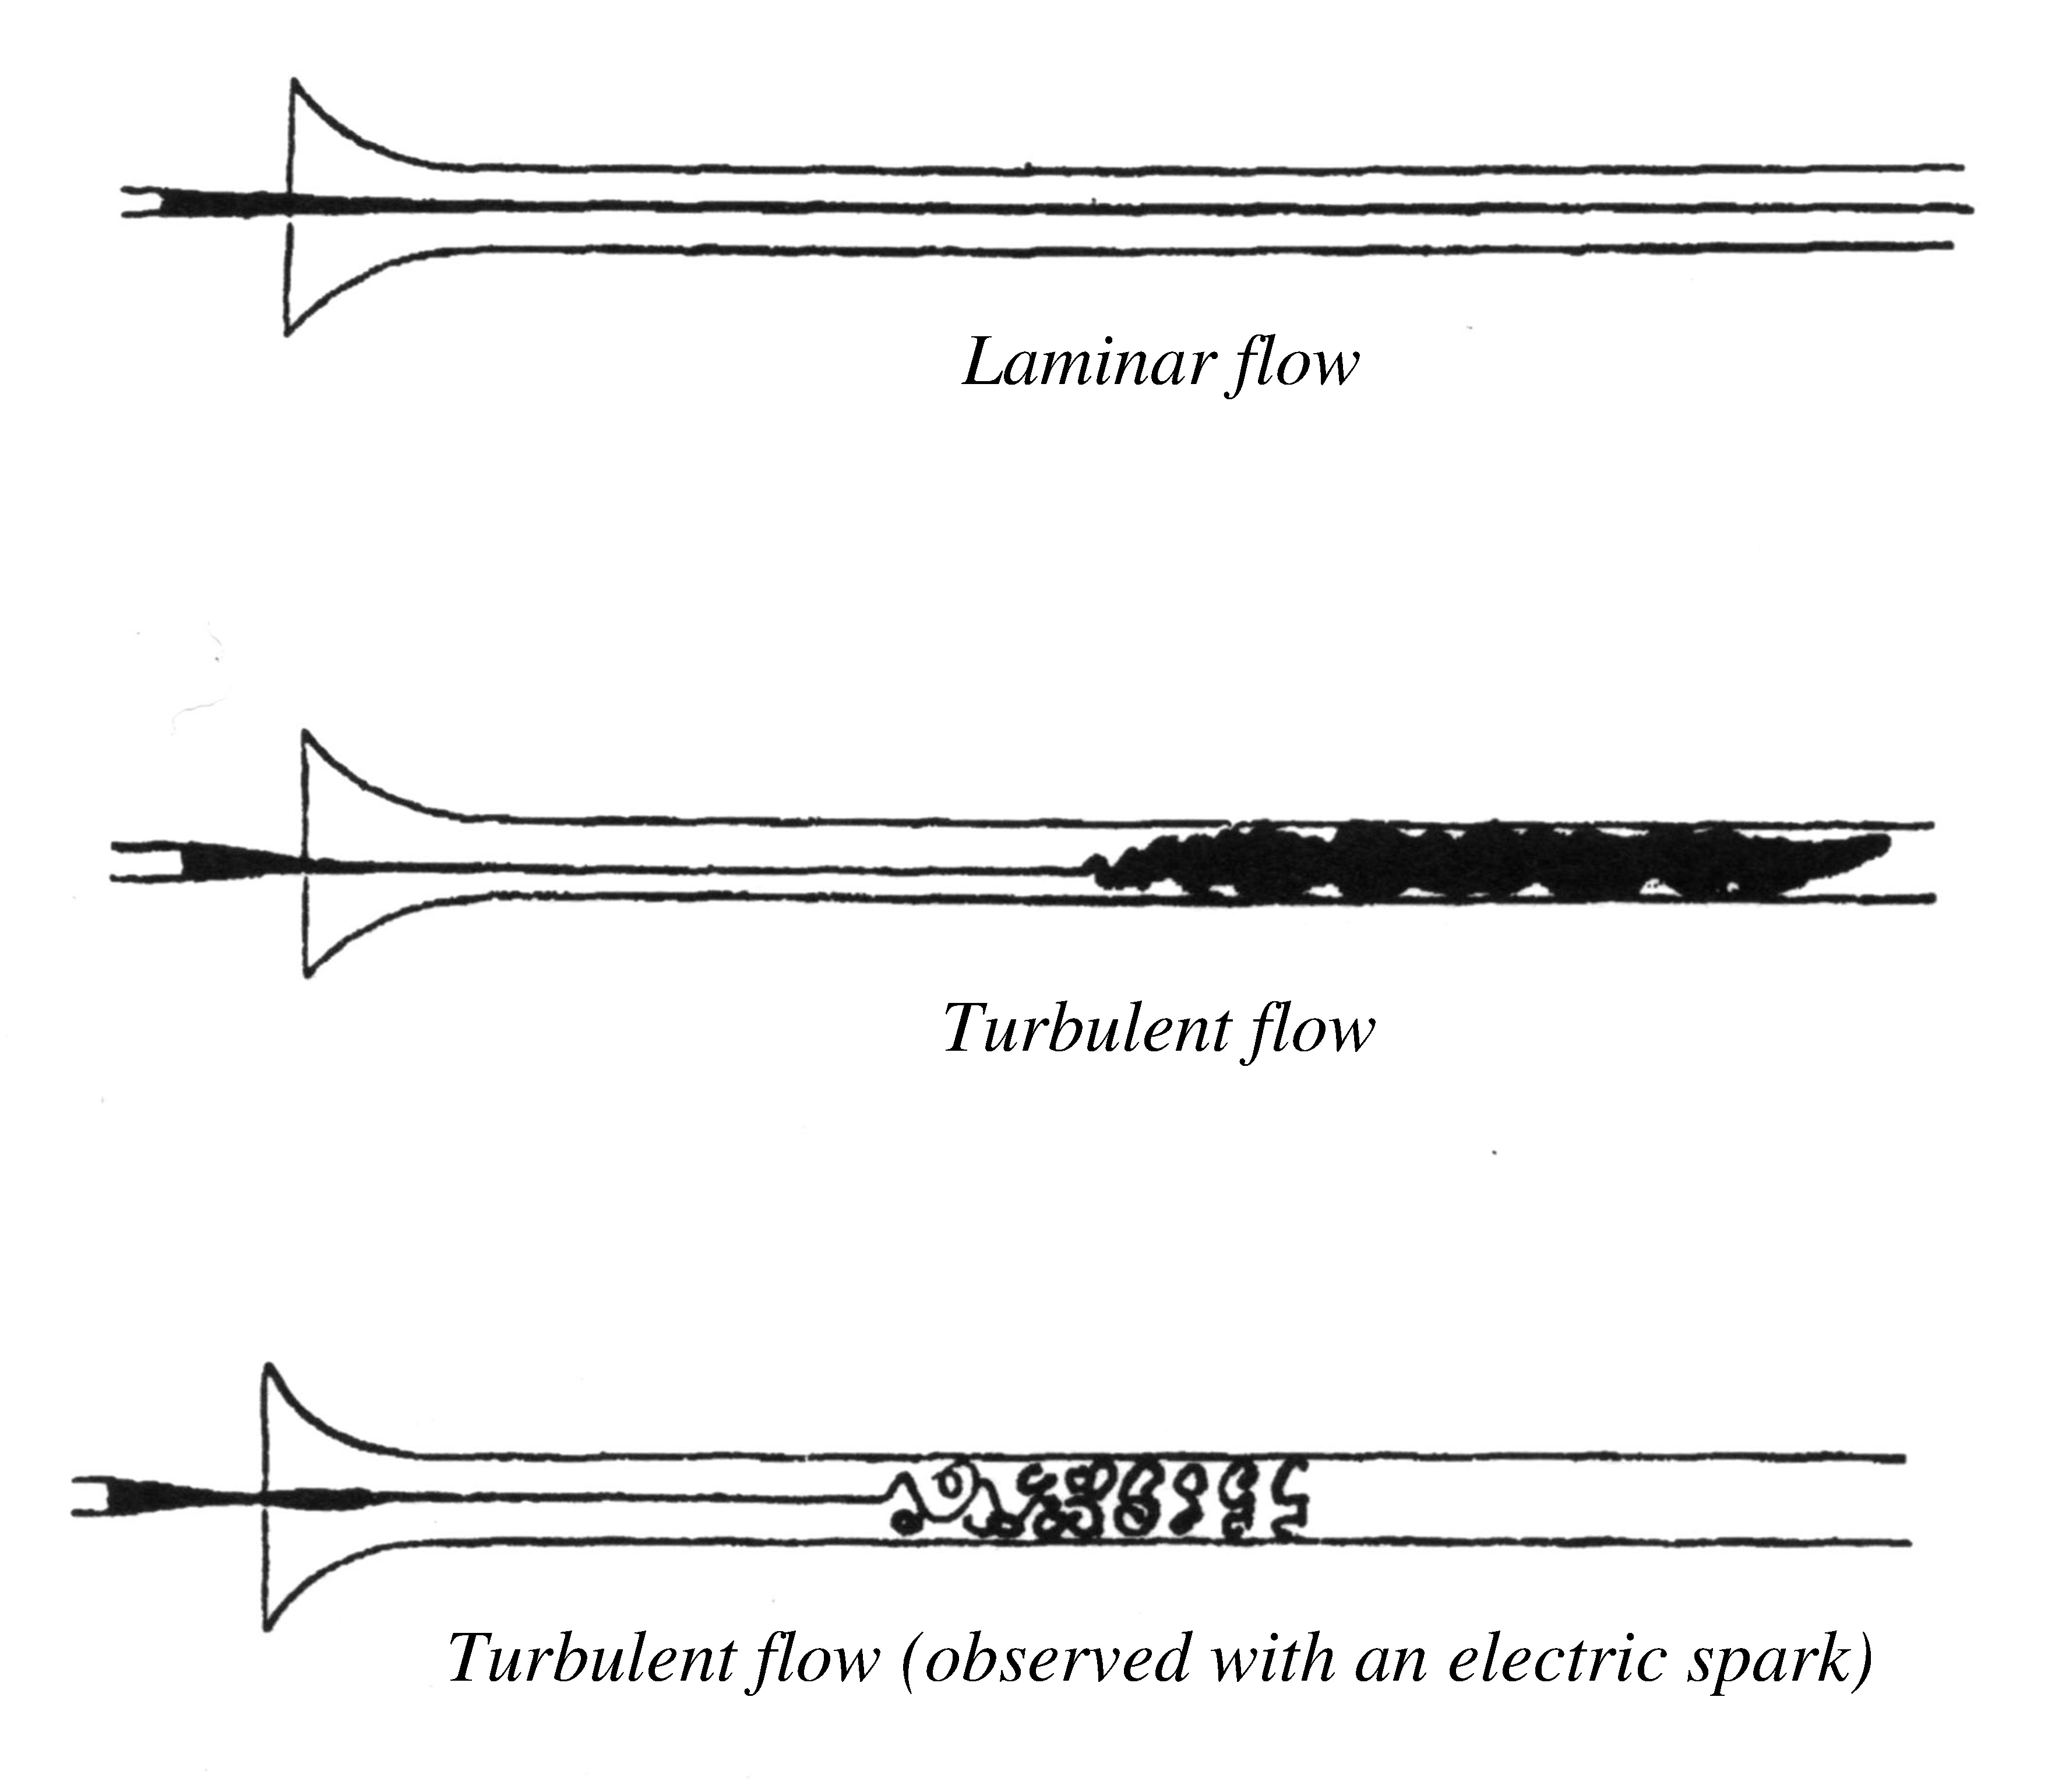
\includegraphics[width=0.5\textwidth]{clase02/Re_observacion.pdf}
\caption{Resultados de Reynolds. Arriba: flujo laminar. Al medio: flujo turbulento. Abajo: flujo turbulento observado con una chispa eléctrica.}
\label{fig:Re_observacion}
\end{figure}

Reynolds concluyó que el flujo cambia de laminar a turbulento a $Re$ entre 2000 y 13000, dependiendo del cuidado que se tiene en la disrupción del flujo (ya sea por tener entradas muy abruptas, como vibraciones).
Esto es algo que podíamos imaginar a partir del análisis que hicimos de la ecuación de Navier-Stokes adimensionalizada.

Para estudiar las estructuras que aparecen en la transición a la turbulencia vamos a utilizar el flujo sobre una placa como nuestro problema modelo.
Cabe destacar que el flujo sobre una placa plana genera lo que se conoce como una capa límite. 
Capa límite es un tema que no hemos pasado en este curso aún, pero solamente es necesario saber que el fluido tendrá velocidad 0 sobre la placa, y irá paulatinamente creciendo a medida que nos alejamos de ella hasta llegar a la velocidad con que viene el flujo al infinito $U_\infty$, como lo muerstra la Figura \ref{fig:capa_limite}.
%
\begin{figure}[h!]
\centering
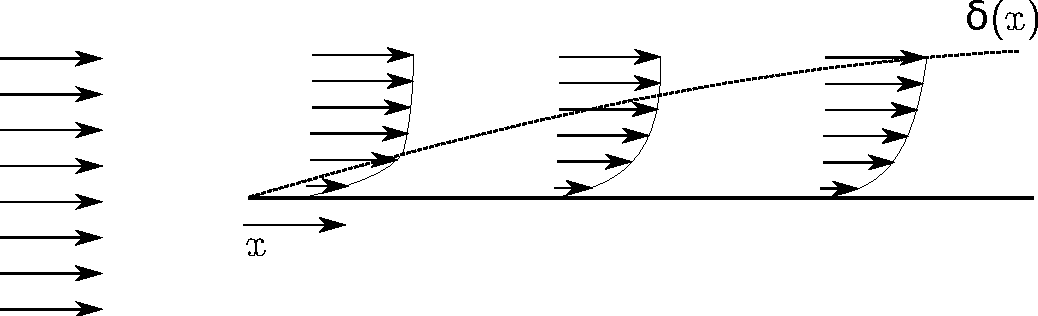
\includegraphics[width=0.5\textwidth]{clase02/capa_limite.pdf}
\caption{Velocidad sobre una placa plana.}
\label{fig:capa_limite}
\end{figure}

Visto desde arriba, la capa límite hace una transición a turbulencia de la forma que muestra la Figura \ref{fig:transicion_turbulencia}.
A continuación haremos una pequeña descripción de cada una de estas etapas.
%
\begin{figure}[h!]
\centering
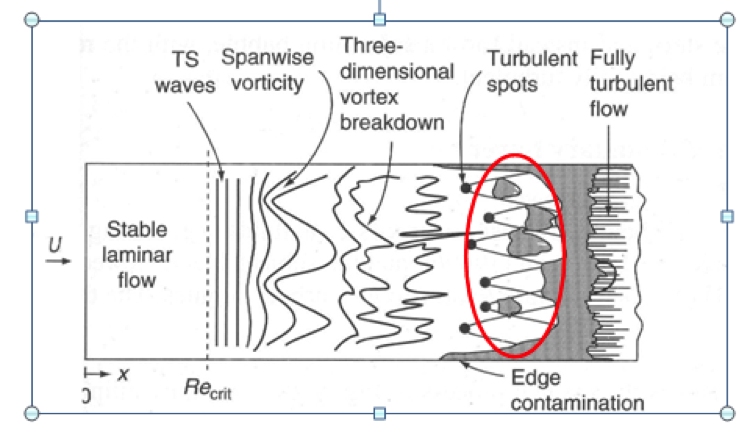
\includegraphics[width=0.5\textwidth]{clase02/transicion_turbulencia.png}
\caption{Transición a turbulencia sobre una placa plana. \emph{Fuente: F. White, Viscous Fluid Flow (2006)}}
\label{fig:transicion_turbulencia}
\end{figure}

\paragraph*{Ondas de Tollmien-Schlichting}
Es la primera indicación de inestabilidad del flujo laminar. 
Estas ondas tienen una naturaleza bidimiensional, ya que son relativamente constantes a lo largo del eje que cruza a lo ancho de la placa.
Inicialmente son prácticamente imperceptibles, pero van creciendo aguas abajo hasta que las nolinealidades de la ecuación de Navier-Stokes comienzan a hacerse notar, generando movimientos en otras direcciones.
Las ondas T-S llegan a ser de \~1-2\% de $U_\infty$.

\paragraph*{Vorticidad a lo ancho de la placa}
Debido a que la no-linealidad toma fuerza, se pierde la bidimiensionalidad del flujo bajo las ondas T-S, y comenzamos a ver variaciones en la vorticidad a lo ancho de la placa.
Inicialmente las variaciones son pequeñas, sin embargo rápidamente toman fuerza y las diferencias en vorticidad a lo largo una misma línea que va hacia adentro puede ser 4 a 5 veces.
Eventualmente, las líneas de vorticidad se tornan irregulares, con vorticidad que se alinea con las líneas de flujo.

\paragraph*{Puntos de turbulencia}
Es la última etapa antes de la turbulencia total.
Las líneas de vorticidad, que se encuentran estiradas, comienzan a romperse en unidades más pequeñas de forma prácticamente aleatoria. 
La turbulencia aparece en forma de puntos o núcleos en tiempos y ubicaciones aleatorias, y se dispersa aguas abajo en un ángulo entre $8^\circ$ y $10^\circ$.

\section*{La ecuación promediada de Reynolds}

Un flujo turbulento es inherentemente desordenado, sin embargo, se puede estudiar viéndolo como un flujo promedio con fluctuaciones aleatorias sobrepuestas.
De esta forma, si medimos la velocidad en un punto determinado, tendríamos algo así como lo que muestra la Figura \ref{fig:flujo_promedio}, que es muy desordenado, pero sigue un promedio.

\begin{figure}[h!]
\centering
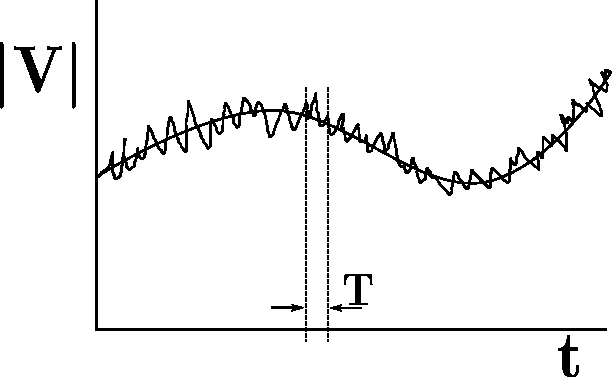
\includegraphics[width=0.5\textwidth]{clase02/flujo_promedio.pdf}
\caption{Medición de velocidad en un punto de un flujo turbulento.}
\label{fig:flujo_promedio}
\end{figure}

Viendo la Figura \ref{fig:flujo_promedio} se hace patente que una buena forma de describir el flujo es superponer fluctuaciones a un promedio.
Estas fluctuaciones mejoran la capacidad de mezcla, difusión y disipación de un flujo, ya que existe una mayor convección.
Por ejemplo, una forma de acelerar la disolución de azucar en un café es revolviéndolo: la turbulencia que uno genera al revolver mueve el azucar dentro de la taza haciendo la ``mezcla'' más eficiente.

Si promediamos la velocidad en un intervalo de tiempo $T$, la velocidad promedio es
%
\begin{equation}
\overline{u} = \frac{1}{T}\int_{t_0}^{t_0+T}udt
\end{equation}
%
donde elegimos el intervalo $T$ tal que sea mayor que cualquier periodo de fluctuación de $u$.
Así, definimos las fluctuaciones de $u$ como $u'$, tal que 
%
\begin{equation} \label{eq:fluctuacion}
u'=u-\overline{u},
\end{equation}
%
y
\begin{equation}
\overline{u'} = 0.
\end{equation}

El promedio de las fluctuaciones es cero porque toma valores positivos y negativos, sin embargo, esto no es muy representativo de la magnitud de las fluctuaciones. 
Para tener una mejor idea de esto, usamos el promedio de su valor al cuadrado
%
\begin{equation}
\overline{u'^2} = \frac{1}{T}\int_{t_0}^{t_0+T} u'^2dt,
\end{equation}
%
y la raíz de este valor que corresponde a la media cuadrática $u'_{RMS} = \sqrt{\overline{u'^2}}$.
Si el valor de $u'_{RMS}$ es independiente del inicio del intervalo $t_0$, se dice que las fluctuaciones son estadísticamente estacionarias.

Formulemos las leyes de conservación usando valores promediados y fluctuaciones.
Primero, escribamos las variables de esta manera:
%
\begin{align}
u &= \overline{u} + u',\quad v = \overline{v} + v',\nonumber\\
w &= \overline{w} + w',\quad p = \overline{p} + p',\
\end{align}
%
con las siguientes propiedades, válidas para cualquier función turbulenta $f$ y $g$
%
\begin{align}\label{eq:promedio_prop}
\overline{f'} &= 0, \quad \overline{\overline{f}}=\overline{f},\quad \overline{f\overline{g}}=\overline{f}\overline{g,} \nonumber\\
\overline{f'\overline{g}} &= 0,\quad \overline{f+g} = \overline{f} +\overline{g},\quad \overline{\frac{\partial f}{\partial s}} = \frac{\partial\overline{f}}{\partial s} \nonumber\\
\overline{\int f ds} &= \int\overline{f}ds,\quad \overline{fg} = \overline{f}\overline{g}+\overline{f'g'}.
\end{align}

Las propiedades en la ecuación \eqref{eq:promedio_prop} son fácilmente demostrables considerando que el promedio es una integral, y por ende, un operador lineal.
Nos daremos el tiempo de demostrar la última propiedad que es un poco menos clara, y además repasaremos demostraciones de otras propiedades en el camino.
%
\begin{align}
\overline{fg} &= \frac{1}{T}\int_{t_0}^{t_0+T}(\overline{f}+f')(\overline{g}+g')dt\nonumber\\
             &= \frac{1}{T}\left(\int_{t_0}^{t_0+T} \overline{f}\overline{g}dt + \int_{t_0}^{t_0+T} \overline{f}g'dt +\int_{t_0}^{t_0+T} f'\overline{g}dt + \int_{t_0}^{t_0+T}f'g'dt\right), \nonumber\\
\text{ pero, }&\int_{t_0}^{t_0+T} f'\overline{g}dt = \overline{g}\int_{t_0}^{t_0+T} f'dt = 0 \text{ (demostrando la cuarta propiedad) }\nonumber\\
\Rightarrow\overline{fg} &= \overline{\overline{f}\overline{g}} + \overline{f'g'} = \overline{f}\overline{g} + \overline{f'g'}
\end{align}

\paragraph*{Conservación de masa.}
En el caso incompresible, la ecuación de continuidad es $\nabla\cdot\mathbf{V}=0$.
Si sacamos el promedio a eso, llegamos a
%
\begin{align}\label{eq:continuidad_prom}
\overline{\frac{\partial u}{\partial x} + \frac{\partial v}{\partial y} + \frac{\partial w}{\partial z}} = 0\nonumber\\
\frac{\partial \overline{u}}{\partial x} + \frac{\partial \overline{v}}{\partial y} + \frac{\partial \overline{w}}{\partial z} = 0.
\end{align}
%
Si a la ecuación de continuidad no promediada, le restamos la Ec. \eqref{eq:continuidad_prom}, llegamos a
%
\begin{equation}\label{eq:continuidad_fluc}
\frac{\partial u'}{\partial x} + \frac{\partial v'}{\partial y} + \frac{\partial w'}{\partial z} = 0
\end{equation}
%
Esto nos indica que tanto el promedio de la velocidad como sus fluctuaciones satisfacen la ecuación de continuidad por si solos para el caso incompresible.

\paragraph*{Conservación de cantidad de movimiento.}
Siguiendo con la suposición de flujo incompresible, saquemos el promedio de la ecuación de Navier-Stokes.
Para esta demostración, usaremos la ecuación de Navier-Stokes en dirección $x$, pero esto es extensible a las otras direcciones.
%
\begin{align}\label{eq:RANS_prev}
\overline{\frac{\partial u}{\partial t} + u\frac{\partial u}{\partial x} + v\frac{\partial u}{\partial y} + w\frac{\partial u}{\partial z}} = \overline{-\frac{1}{\rho}\frac{\partial p}{\partial x} + \nu\left(\frac{\partial^2u}{\partial x^2}+ \frac{\partial^2u}{\partial y^2}+\frac{\partial^2u}{\partial z^2}\right)}\nonumber\\
\frac{\partial \overline{u}}{\partial t} + \overline{u\frac{\partial u}{\partial x}} + \overline{v\frac{\partial u}{\partial y}} + \overline{w\frac{\partial u}{\partial z}} = -\frac{1}{\rho}\frac{\partial \overline{p}}{\partial x} + \nu\left(\frac{\partial^2\overline{u}}{\partial x^2}+ \frac{\partial^2\overline{u}}{\partial y^2}+\frac{\partial^2\overline{u}}{\partial z^2}\right)
\end{align}
%
El paso que hicimos acá es bastante directo: la suma, derivada e integral (promedio) son operaciones lineales y uno puede intercambiarlas de orden (por ejemplo, $\overline{\frac{\partial u}{\partial x}} = \frac{\partial\overline{u}}{\partial x}$).
Los términos más complicados son los no lineales; desarrollemos uno de ellos:
%
\begin{align}
\overline{v\frac{\partial u}{\partial y}} &= \overline{(\overline{v}+v')\frac{\partial}{\partial y}(\overline{u}+u')} = \overline{\overline{v}\frac{\partial\overline{u}}{\partial y}} + \overline{\overline{v}\frac{\partial u'}{\partial y}} + \overline{v'\frac{\partial\overline{u}}{\partial y}} + \overline{v'\frac{\partial u'}{\partial y}} \nonumber\\
&\text{pero, }\overline{\overline{v}\frac{\partial u'}{\partial y}} = \overline{v'\frac{\partial\overline{u}}{\partial y}}=0, \nonumber\\
\Rightarrow&\overline{v\frac{\partial u}{\partial y}}= \overline{v}\frac{\partial\overline{u}}{\partial y} + \overline{v'\frac{\partial u'}{\partial y}}.
\end{align}

La notación que estamos usando es quizás no muy conveniente, por que tenemos que escribir mucho.
Si usamos notación indicial, en una ecuación podemos resumir todo. 
Llamemos al vector $\mathbf{V} = (u,v,w) = (u_1,u_2,u_3)$, donde $u_1=u$, $u_2=v$ y $u_3=w$ y $\mathbf{x} = (x,y,z) = (x_1,x_2,x_3)$.
Podemos escribir la ecuación \eqref{eq:RANS_prev} como
%
\begin{equation}\label{eq:RANS_prev2}
\frac{\partial \overline{u}_i}{\partial t} + \overline{u}_j\frac{\partial \overline{u}_i}{\partial x_j} + \overline{u_j'\frac{\partial u'_i}{\partial x_j}} = -\frac{1}{\rho}\frac{\partial \overline{p}}{\partial x_i} + \nu \frac{\partial}{\partial x_j}\frac{\partial \overline{u}_i}{\partial x_j},
\end{equation}
%
donde $i=1,2,3$ y $j=1,2,3$. 
La convención dice que si un índice se repite en un término, éste es una suma.
Por ejemplo, $\frac{\partial u_i}{\partial x_i}=\frac{\partial u_1}{\partial x_1} + \frac{\partial u_2}{\partial x_2} + \frac{\partial u_3}{\partial x_3}$ es otra forma de escribir la divergencia de la velocidad.

Usando el hecho de que el flujo es incompresible, y la divergencia de las fluctuaciones es cero ($\partial u'_i/\partial x_i=0$), podemos escribir:
%
\begin{equation}
\overline{u_j'\frac{\partial u_i}{\partial x_j}} = \overline{u_j'\frac{\partial u'_i}{\partial x_j} + u_i'\frac{\partial u'_j}{\partial x_j}} = \overline{\frac{\partial u_i'u_j'}{\partial x_j}} = \frac{\partial \overline{u_i'u_j'}}{\partial x_j}
\end{equation}
%
y la Ec. \eqref{eq:RANS_prev2} queda
%
\begin{equation}\label{eq:RANS}
\frac{\partial \overline{u}_i}{\partial t} + \overline{u}_j\frac{\partial \overline{u}_i}{\partial x_j} + \frac{\partial \overline{u'_iu'_j}}{\partial x_j} = -\frac{1}{\rho}\frac{\partial \overline{p}}{\partial x_i} + \nu \frac{\partial}{\partial x_j}\frac{\partial \overline{u}_i}{\partial x_j},
\end{equation}

La Ec. \eqref{eq:RANS} se conoce como la ecuación de Reynolds.
La ecuación de Reynolds es muy parecida a la ecuación de Navier-Stokes con cada término promedidado por si solo, más $\frac{\partial \overline{u'_iu'_j}}{\partial x_j}$.
El término $\overline{u'_iu'_j}$ se conoce como el tensor de esfuerzos de Reynolds \mbox{?`}Por qué tensor? $i$ y $j$ pueden tomar tres valores (1, 2 o 3), por lo que existen 9 posibles valores, que podemos ordenar en una matriz $3\times 3$.
Es el tensor de esfuerzos de Reynolds el que produce todas las complicaciones en el estudio de turbulencia, y se ha gastado mucho tiempo y recursos en generar ecuaciones que nos permitan modelar este término.

\begin{figure}[h!]
\centering
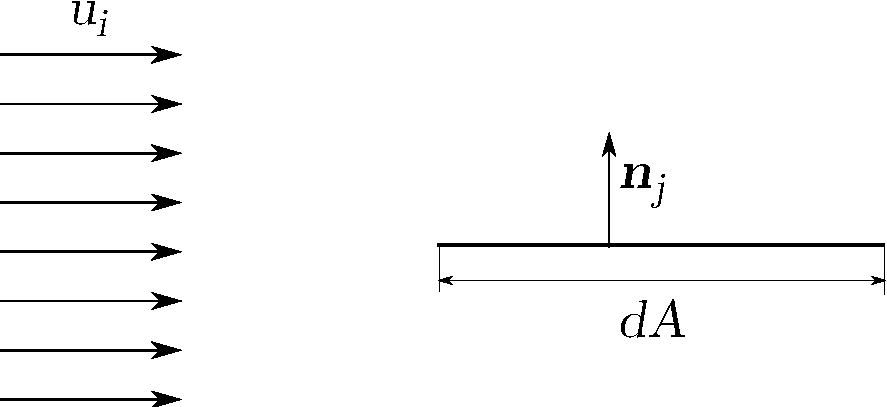
\includegraphics[width=0.5\textwidth]{clase02/flujo_momentum.pdf}
\caption{Flujo de momentum en un flujo turbulento}
\label{fig:flujo_momentum}
\end{figure}
%
El nombre tensor de esfuerzos no parece ser muy adecuado, ya que son solamente términos de la inercia turbulenta, no esfuerzos.
Sin embargo, podemos visualizar este tensor como un esfuerzo, pues genera un flujo de momentum.
Usemos la Figura \ref{fig:flujo_momentum} para ejemplificar esto.
Esta figura presenta un flujo uniforme turbulento con velocidad en el eje $i$, $u_i = \overline{u}_i + u'_i$, y un área $dA$ alineada con el flujo (su normal es perpendicular a $i$, $\mathbf{n}_j$).
La cantidad de fluido que pasa por $dA$ en un tiempo $dt$ es igual a $u_jdAdt$, y el caudal $Q=u_jdA$, pero el flujo promedio no tiene componente en el eje $j$, por lo tanto, $\overline{u}_j=0$ y $u_j = u'_j$.
El flujo de cantidad de movimiento en el eje $i$ que pasa por $dA$ entonces es 
%
\begin{equation}
\frac{dp_i}{dt} = \rho u_i \rho \mathbf{u}\cdot\mathbf{n}_j dA = \rho u_i Q = \rho u_i u'_j dA.
\end{equation}
%
En un flujo turbulento las cantidades instantáneas no nos dicen mucho, saquemos el promedio
%
\begin{equation}
\frac{d\overline{p}_i}{dt} = \rho \overline{u_i u'j} dA = \rho \overline{u'_iu'_j}dA.
\end{equation}
%
Esto nos indica que el tensor de esfuerzo de Reynolds está presente en el cálculo del flujo de cantidad de movimiento, sin embargo, sigue sin ser un esfuerzo.

Podemos escribir el tensor de Reynolds como si fueran esfuerzos si generamos la variable $\tau$, tal que:
%
\begin{equation}
\tau_{ij} = \mu\left(\frac{\partial u_i}{\partial x_j} + \frac{\partial u_j}{\partial x_i}\right) - \rho \overline{u_i'u_j'},
\end{equation}
%
y lo pasamos al lado derecho de la ecuación:
%
\begin{equation}\label{eq:tensor}
\rho\frac{\partial \overline{u}_i}{\partial t} + \rho\overline{u}_j\frac{\partial \overline{u}_i}{\partial x_j} +  = -\frac{\partial \overline{p}}{\partial x_i} + \frac{\partial}{\partial x_j}\tau_{ij},
\end{equation}



\subsection*{Energía cinética turbulenta}
En el afán de comprender la turbulencia de mejor manera, se ha intentado agregar algo así como ``leyes de conservación turbulenta''.
La más obvia de estas es la energía cinética turbulenta, que esla energía cinética debido a las fluctuaciones turbulentas:
%
\begin{equation}
K = \frac{1}{2}\left( \overline{u'u'}+\overline{v'v'}+\overline{w'w'}\right)=\frac{1}{2}\overline{u'_iu'_i}
\end{equation}

Podemos derivar una ley de conservación de energía cinética desde la ecuación de Navier-Stokes al hacer el producto punto con $\mathbf{V}$, sacando el promedio de esa ecuación, y restándole ese promedio a la ecuación original. 
Después de bastante algebra, llegamos a
%
\begin{align}\label{eq:K_conservacion}
\frac{DK}{Dt} =& -\frac{\partial}{\partial x_i} \left[ \overline{u'_i\left(\frac{1}{2}u'_iu'_j+\frac{p'}{\rho}\right)}\right] - \overline{u'_iu'_j}\frac{\partial\overline{u}_j}{\partial x_i} \nonumber\\
               & + \frac{\partial}{\partial x_i}\left[\overline{\nu u_j'\left(\frac{\partial u'_i}{\partial x_j} + \frac{\partial u_j'}{\partial x_i}\right)}\right] -\nu\overline{\frac{\partial u_j'}{\partial x_i}\left(\frac{\partial u_i'}{\partial x_j}+\frac{\partial u_j'}{\partial x_i}\right)}
\end{align}

La Ec. \eqref{eq:K_conservacion} es tremendamente complicada, pero hay algunas cosas que podemos sacar en limpio, sobre todo si la integramos en un volúmen fijo en el espacio.
El término a la izquierda es la derivada material, en otras palabras, la razón de cambio de $K$ en un elemento de fluido que se mueve con el flujo.
Al integrar el segundo término, podemos utilizar el teorema de la divergencia para visualizarlo como convección de energía cinética a través de la superficie.
El tercer término no tiene una forma que se pueda asociar a un proceso de convección o difusión, y puede ser visto como una fuente, o producción de energía cinética.
El cuarto término también toma importancia en el borde del volumen de integración con el teorema de la divergencia, y es el trabajo realizado por los esfuerzos viscosos en ese borde.
Finalmente el quinto es la disipación viscosa.



